% Encoding: UTF-8
%%%%%%%%%%%%%%%%%%%%%%%%%%%%%%%%%%%%%%%%%%%%%%%%%%%%%%%%%%%%%%%%%%%%%%%%%%%%%%%

%%%%%%%%%%%%%%%%%%%%%%%%%%%%%%%%%%%%%%%%%%%%%%%%%%%%%%%%%%%%%%%%%%%%%%%%%%%%%%%
% $Id: slides.tex 17 2011-02-10 15:21:56Z klugeflo $
%%%%%%%%%%%%%%%%%%%%%%%%%%%%%%%%%%%%%%%%%%%%%%%%%%%%%%%%%%%%%%%%%%%%%%%%%%%%%%%

%%%%%%%%%%%%%%%%%%%%%%%%%%%%%%%%%%%%%%%%%%%%%%%%%%%%%%%%%%%%%%%%%%%%%%%%%%%%%%%
%%
%% Vorlage fuer LaTeX-Beamer
%% gemaess dem Corporate Design der Uni Augsburg
%%
%%%%%%%%%%%%%%%%%%%%%%%%%%%%%%%%%%%%%%%%%%%%%%%%%%%%%%%%%%%%%%%%%%%%%%%%%%%%%%%
%%
%% Changelog:
%%
%% 11/02/10 (FAK) Start
%%
%%%%%%%%%%%%%%%%%%%%%%%%%%%%%%%%%%%%%%%%%%%%%%%%%%%%%%%%%%%%%%%%%%%%%%%%%%%%%%%


%%%%%%%%%%%%%%%%%%%%%%%%%%%%%%%%%%%%%%%%%%%%%%%%%%%%%%%%%%%%%%%%%%%%%%%%%%%%%%%

\documentclass[xcolor=pdftex,dvipsnames,table]{beamer}

%%%%%%%%%%%%%%%%%%%%%%%%%%%%%%%%%%%%%%%%%%%%%%%%%%%%%%%%%%%%%%%%%%%%%%%%%%%%%%%

% Language settings
% IMPORTANT: If you change the language settings, make sure to run
% cleantex prior to any latex/pdflatex to remove all .aux files, else
% latex might fail!
%\usepackage[english]{babel}
\usepackage[german]{babel}

%\usepackage{graphicx}
\usepackage[utf8]{inputenc}
%\usepackage{mathptmx}

\usepackage{svg}
\usepackage{textcomp}
\usepackage{german}
\usepackage{tikz}
\usepackage{pgfplots}
\usepackage{booktabs}% http://ctan.org/pkg/booktabs
\newcommand{\tabitem}{~~\llap{\textbullet}~~}
\usetikzlibrary{automata,positioning}
\usetikzlibrary{arrows,automata,shapes,calc}


\graphicspath{{./img/}}
%%%%%%%%%%%%%%%%%%%%%%%%%%%%%%%%%%%%%%%%%%%%%%%%%%%%%%%%%%%%%%%%%%%%%%%%%%%%%%%

\usetheme{fai}

% IMPORTANT/TODO: currently only PDF graphic files should be used, PNG
% or JPEG may harm the Adobe Reader colour palette and result in
% strange display colours.
%\DeclareGraphicsExtensions{.pdf}

%\graphicspath{{./img/}}

%%%%%%%%%%%%%%%%%%%%%%%%%%%%%%%%%%%%%%%%%%%%%%%%%%%%%%%%%%%%%%%%%%%%%%%%%%%%%%%
%% Presentation main settings
%%%%%%%%%%%%%%%%%%%%%%%%%%%%%%%%%%%%%%%%%%%%%%%%%%%%%%%%%%%%%%%%%%%%%%%%%%%%%%%

\title{Handschrifterkennung mit CUDA und C++}
%\subtitle{Optional Subtitle}
\author{Christopher Haug, Dominik Walter}
\institute[Uni Augsburg]{University of Augsburg\\Systems and Networking}
\date[]{\today}


%%%%%%%%%%%%%%%%%%%%%%%%%%%%%%%%%%%%%%%%%%%%%%%%%%%%%%%%%%%%%%%%%%%%%%%%%%%%%%%
%% Main Document starts here
%%%%%%%%%%%%%%%%%%%%%%%%%%%%%%%%%%%%%%%%%%%%%%%%%%%%%%%%%%%%%%%%%%%%%%%%%%%%%%%
\setbeamertemplate{section in toc}[ball]
\setbeamertemplate{subsection in toc}[ball unnumbered]
\setbeamertemplate{subsubsection in toc}[ball unnumbered]
\AtBeginSection []{
	\begin{frame}
		\frametitle{Inhaltsverzeichnis}
		\tableofcontents[currentsection,subsubsectionstyle={show/show/show/shaded}]
	\end{frame}
}

\AtBeginSubsection []{
	\begin{frame}
		\frametitle{Inhaltsverzeichnis}
		\tableofcontents[currentsection,subsectionstyle={show/shaded/shaded}]
	\end{frame}
}

\AtBeginSubsubsection []{
	\begin{frame}
		\frametitle{Inhaltsverzeichnis}
		\tableofcontents[currentsection,subsectionstyle={show/shaded/shaded},subsubsectionstyle={show/shaded/shaded/shaded}]
	\end{frame}
}

\begin{document}
	\frame{\titlepage}
	\begin{frame}
		\frametitle{Aufgabe}
		\begin{columns}
			\begin{column}{0.25\textwidth}
				
\includegraphics[width=1\textwidth]{sample.png}
			\end{column}
			\begin{column}{0.05\textwidth}
				\\
				
\includegraphics[width=1\textwidth]{arrow.png}\\
				
\includegraphics[width=1\textwidth]{arrow.png}\\
				
\includegraphics[width=1\textwidth]{arrow.png}\\
				
\includegraphics[width=1\textwidth]{arrow.png}\\
				
\includegraphics[width=1\textwidth]{arrow.png}\\
				
\includegraphics[width=1\textwidth]{arrow.png}
			\end{column}
			\begin{column}{0.4\textwidth}
				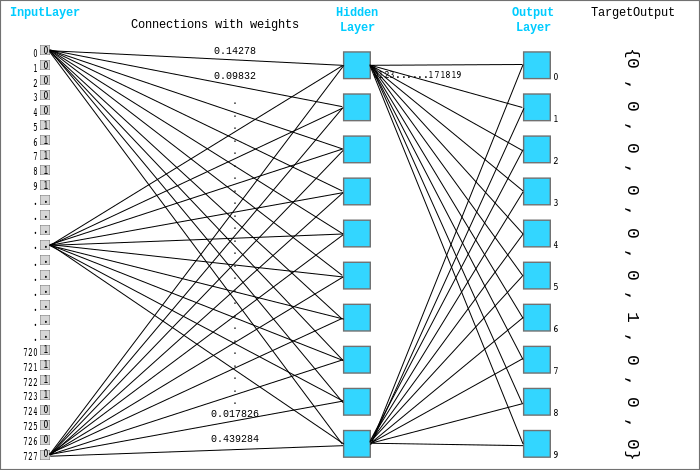
\includegraphics[width=1\textwidth]{nn.png}
			\end{column}
			\begin{column}{0.05\textwidth}
				\\
				
\includegraphics[width=1\textwidth]{arrow.png}\\
				
\includegraphics[width=1\textwidth]{arrow.png}\\
				
\includegraphics[width=1\textwidth]{arrow.png}\\
				
\includegraphics[width=1\textwidth]{arrow.png}\\
				
\includegraphics[width=1\textwidth]{arrow.png}\\
				
\includegraphics[width=1\textwidth]{arrow.png}
			\end{column}
			\begin{column}{0.25\textwidth}
				
\includegraphics[width=1\textwidth]{prediction.png}
			\end{column}
		\end{columns}
	\LARGE
		\begin{itemize}
			\item Erkennung von handgeschriebenen Zahlen
			\item Neuronales Netz
			\item CUDA und C++
		\end{itemize}
		
	\end{frame}
	
	\begin{frame}
		\frametitle{Training/Testing Dataset}
		\begin{block}{THE MNIST DATABASE of handwritten digits}
		\tabitem 60.000 Trainings-Bilder\\
		\tabitem 10.000 Test-Bilder\\
		\tabitem Auflösung: 28x28\\
		\tabitem IDX-Format\\
		\tabitem Source: http://yann.lecun.com/exdb/mnist/
		\end{block}
		
\includegraphics[width=0.15\textwidth]{trainings_sample_example_0.png}
		
\includegraphics[width=0.15\textwidth]{trainings_sample_example_1.png}
		
\includegraphics[width=0.15\textwidth]{trainings_sample_example_2.png}
		
\includegraphics[width=0.15\textwidth]{trainings_sample_example_3.png}
		
\includegraphics[width=0.15\textwidth]{trainings_sample_example_4.png}\\
		
\includegraphics[width=0.15\textwidth]{trainings_sample_example_5.png}
		
\includegraphics[width=0.15\textwidth]{trainings_sample_example_6.png}
		
\includegraphics[width=0.15\textwidth]{trainings_sample_example_7.png}
		
\includegraphics[width=0.15\textwidth]{trainings_sample_example_8.png}
		
\includegraphics[width=0.15\textwidth]{trainings_sample_example_9.png}
		
	\end{frame}


	\begin{frame}
		\frametitle{Feed-Forward / Back-Propagation}
		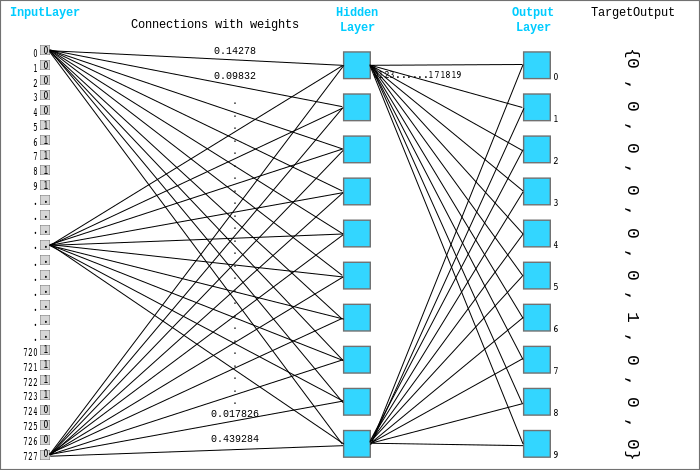
\includegraphics[width=1\textwidth]{nn.png}
	\end{frame}

	\begin{frame}
		\frametitle{CUDA-Implementierung}
		\begin{columns}
			\begin{column}{0.5\textwidth}
				\underline{Feed-Forward:}
				\begin{itemize}
					\item Eingabe-Kanten (edges)
					\begin{itemize}
						\item Thread
						\item Berechnet Kanten-Wert
						\item Speichert in $Shared Memory$
					\end{itemize}
					\item Knoten (nodes)
					\begin{itemize}
						\item Thread-Block
						\item Summiert alle Kanten-Werte
						\item Berechnet Knoten-Wert (Sigmoid)
					\end{itemize}
					\item Ausgabe
					\begin{itemize}
						\item Index des höhsten Knoten im $OutputLayer$
					\end{itemize}
				\end{itemize}
			\end{column}
			\begin{column}{0.6\textwidth}
				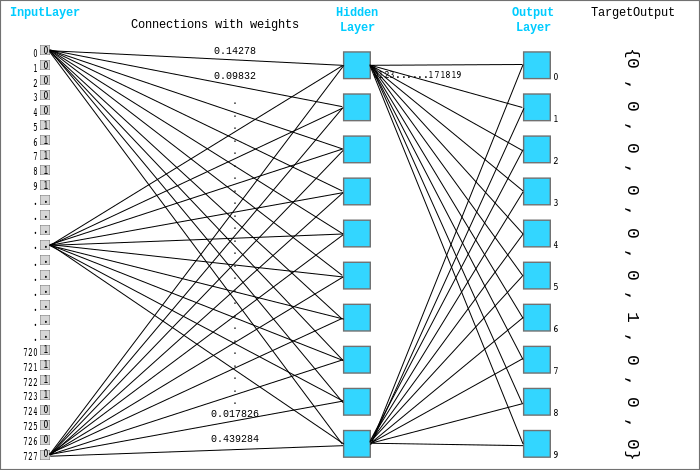
\includegraphics[width=1\textwidth]{nn.png}
			\end{column}
		\end{columns}
	\end{frame}

	\begin{frame}
		\frametitle{CUDA-Implementierung}
		\begin{columns}
			\begin{column}{0.5\textwidth}
				\underline{Back-Propagation:}
				\begin{itemize}
					\item Ausgehende-Kanten (edges)
					\begin{itemize}
						\item Thread
						\item Berechnet Kanten-Fehler
						\item Speichert in $Shared Memory$
						\item Aktualisiert Kanten-Gewichte
					\end{itemize}
					\item Knoten (nodes)
					\begin{itemize}
						\item Thread-Block
						\item Summiert alle Kanten-Fehler
						\item Berechnet Knoten-Fehler
					\end{itemize}
				\end{itemize}
			\end{column}
			\begin{column}{0.6\textwidth}
				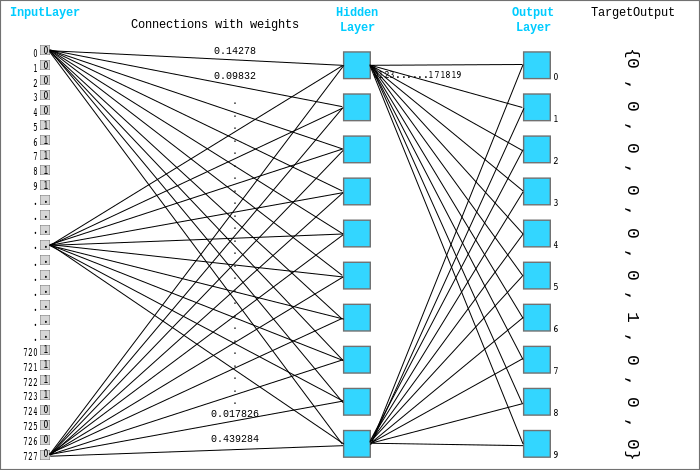
\includegraphics[width=1\textwidth]{nn.png}
			\end{column}
		\end{columns}
	\end{frame}

	\begin{frame}
		\frametitle{C++-Implementierung}
		\begin{columns}
			\begin{column}{0.5\textwidth}
				\begin{itemize}
					\item Aufteilung der Knoten auf n Threads
					\item Jeder Thread berechnet k Knoten-Werte/-Fehler
					\item Bulk-Synchronisation zwischen den Ebenen
				\end{itemize}
			\end{column}
			\begin{column}{0.6\textwidth}
				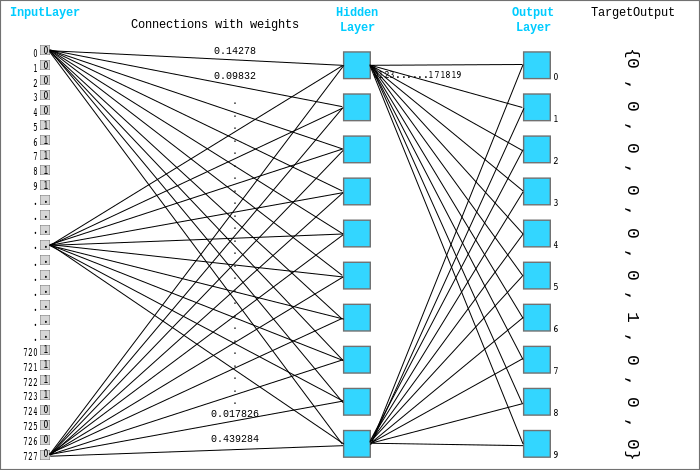
\includegraphics[width=1\textwidth]{nn.png}
			\end{column}
		\end{columns}
	\end{frame}

	\begin{frame}
		\frametitle{Auswertung-Generic TODO}
		\begin{figure}[htbp]
	\begin{minipage}{0.9\textwidth}	
		\begin{tikzpicture}
		\begin{semilogyaxis}[
		width=1\textwidth,
		enlarge x limits={abs=1.5cm},
		height=0.3\textwidth,
		ybar,
		bar width=0.3cm,
		ylabel={TODO},
		xlabel={TODO},
		legend style={at={(0.5,1.05)},anchor=south,legend
			columns=-1},
		symbolic x coords={x, y, z},
		xtick align=inside,
		xtick=data
		]

		\addplot +[area legend] coordinates {
			(x, 205120)	
			(y, 1375)
			(z, 304256)
			
		};

		\addplot +[area legend] coordinates {
			(x, 5995520)
			(y, 156992)
			(z, 27899008)
			
		};

		\addplot +[area legend] coordinates {
			(x, 67793976)	
			(y, 1157136)
			(z, 301377384)
			
		};		
		\legend{
			x,
			y,
			z
		}
		\end{semilogyaxis}
		\end{tikzpicture}
	\end{minipage}
		\begin{figure}[htbp]
	\begin{minipage}{1\textwidth}
		% legend
		\begin{tikzpicture}
		\begin{axis}[
		width=0.87\textwidth,
		height=0.2\textwidth,
		hide axis,
		symbolic x coords={0}
		]

		\addplot +[mark=] coordinates {
			(0,0)
		};

		\addplot +[mark=] coordinates {
			(0,0)
		};

		\addplot +[mark=] coordinates {
			(0,0)
		};
		\legend{a, b}
		\end{axis}
		\end{tikzpicture}
	\end{minipage}
	\begin{minipage}{0.325\textwidth}
		% IS
		\begin{tikzpicture}
		\begin{semilogyaxis}[
		width=1.15\textwidth,
		xlabel={x},
		legend style={at={(0.5,1.05)},anchor=south},
		xtick=data,
		xticklabels={$_2$,$_3$,$_4$,$_2$,2,3,4,2}
		]
		
		
		\addplot +[mark=] coordinates {
			(79, 50617585) (80, 50465035) (81, 52132224) (82, 41708585) (83, 22660009) (84, 22916748) (85, 22811790) (86, 22660009)
		};
	
		\addplot +[mark=] coordinates {
			(79, 34896112) (80, 31484235) (81, 24788262) (82, 31034653) (83, 25894023) (84, 25230307) (85, 24911442) (86, 25894023) 
		};
		
		\end{semilogyaxis}
		\end{tikzpicture}
	\end{minipage}
	%DT
	\begin{minipage}{0.325\textwidth}	
		\begin{tikzpicture}
		\begin{semilogyaxis}[
		width=1.15\textwidth,
		xlabel={y},
		legend style={at={(0.5,1.05)},anchor=south,legend},
		xtick=data,
		xticklabels={$_2$,$_3$,$_4$,$_2$,2,3,4,2}
		]

		\addplot +[mark=] coordinates {
			(79, 2216845) (80, 2312995) (81, 2426046) (82, 2122934) (83, 2126110) (84, 2203558) (85, 2388962) (86, 2126110) 
		};
	
		\addplot +[mark=] coordinates {
			(79, 1966208) (80, 2050492) (81, 2086301) (82, 1963645) (83, 2461961) (84, 2410293) (85, 2563874) (86, 2461961)
		};
		
		\end{semilogyaxis}
		\end{tikzpicture}
	\end{minipage}
	% CG
	\begin{minipage}{0.325\textwidth}
		\begin{tikzpicture}
		\begin{semilogyaxis}[
		width=1.15\textwidth,
		xlabel={z},
		legend style={at={(0.5,1.05)},anchor=south,legend
			columns=-1},
		xtick=data,
		xticklabels={$_2$,$_3$,$_4$,$_2$,2,3,4,2}
		]

		\addplot +[mark=] coordinates {
			(79, 281861317) (80, 253046064) (81, 285023162) (82, 90994546) (83, 91800314) (84, 88307720) (85, 88526507) (86, 91708040)
		};

		\addplot +[mark=] coordinates {
			(79, 129645476) (80, 96242016) (81, 93795705) (82, 92430244) (83, 107873591) (84, 96351507) (85, 96421277) (86, 107856802) 
		};

		\end{semilogyaxis}
		\end{tikzpicture}
	\end{minipage}
\end{figure}
\end{figure}
	\end{frame}

\end{document}
